\documentclass{beamer}
%
% Choose how your presentation looks.
%
% For more themes, color themes and font themes, see:
% http://deic.uab.es/~iblanes/beamer_gallery/index_by_theme.html
%
\mode<presentation>
{
  \usetheme{Madrid}      % or try Darmstadt, Madrid, Warsaw, ...
  \usecolortheme{default} % or try albatross, beaver, crane, ...
  \usefonttheme{default}  % or try serif, structurebold, ...
  \setbeamertemplate{navigation symbols}{}
  \setbeamertemplate{caption}[numbered]
} 

\usepackage[english]{babel}
\usepackage[utf8x]{inputenc}
\usepackage{amsmath}
\usepackage{tcolorbox}
\usepackage{graphicx}
\usepackage{subcaption}
\usepackage{algorithm2e}
\usepackage{apacite}


\title{Robust Single Linkage Algorithm and Extract Flat Clustering}
\author{Taoran Xue}
\institute{George Washington University}

\begin{document}

\begin{frame}
  \titlepage
\end{frame}



\section{Introduction}

\begin{frame}{Introduction}
\begin{itemize}
	\item There are many sources of almost unlimited data:
	\begin{enumerate}
		\item Images from the web.
		\item Speech recorded by a microphone.
		\item Records of credit card or other transactions.
	\end{enumerate}
	\item Noise points occasionally draws between two cluster
\end{itemize}

\end{frame}

\section{Minimum spanning tree}

\begin{frame}{Minimum spanning tree}

\begin{tcolorbox}
	For each $i$, set $r(x_i)$ to the distance from $x_i$ to its {\color{red}$k$}th nearest neighbor.
	
	As $r$ grows from $0$ to $\infty$:
	\begin{enumerate}
		\item Construct a graph $G_r$ with nodes $\{x_i : r(x_i) \leq r\}$. Include edge $(x_i, x_j)$ if $\|x_i - x_j\| \leq$ {\color{red}$\alpha r$}.
		\item Let $\mathbb{C}_n(r)$ be the connected components of $G_r$.
	\end{enumerate}  
	
\end{tcolorbox}


\begin{definition}
	Set $r_k(x_i)$ to the distance to $k$th nearest neighbor. For any $r = \text{max}\{r_k(x_i)\}$, connect points $x_i$ and $x_j$, if $||x_i - x_j|| \leq \alpha r$.
\end{definition}

\end{frame}

\begin{frame}{New distance function}

\begin{figure}[h!]
	\centering
	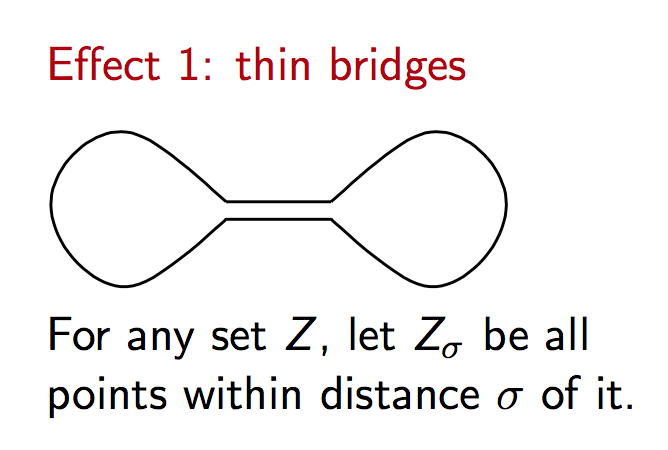
\includegraphics[scale=0.35]{a.png}
	\caption{``Thin bridge'' effect.}
	\label{fig:slabfig}
\end{figure}

\begin{definition}
	Set $core_k(x_i)$ to the distance to $k$th nearest neighbor.
	$$d_{\mathrm{mrd}_k}(x_i, x_j) = \text{max}\{core_k(x_i), core_k(x_j), ||x_i - x_j||\}$$
\end{definition}

\end{frame}

\begin{frame}{Mutual reachability distance}

\begin{definition}
	Set $core_k(x_i)$ to the distance to $k$th nearest neighbor.
	$$d_{\mathrm{mrd}_k}(x_i, x_j) = \text{max}\{core_k(x_i), core_k(x_j), ||x_i - x_j||\}$$
\end{definition}

\begin{figure}[h!]
	\begin{subfigure}{.5\textwidth}
		\centering
		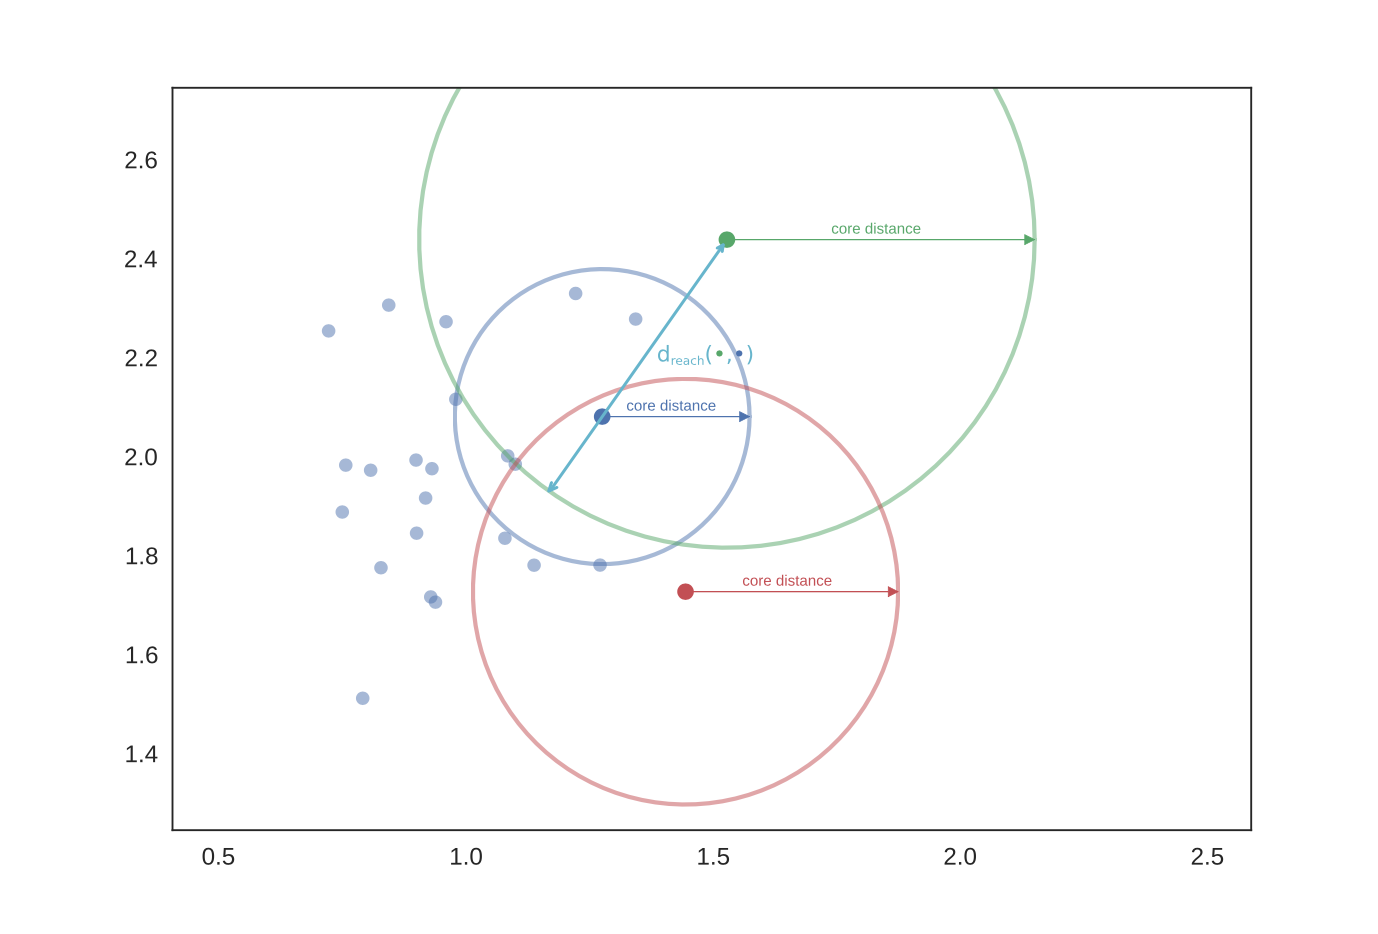
\includegraphics[width=\linewidth]{dis_figure1.png}
		\caption{}
	\end{subfigure}%
	\begin{subfigure}{.5\textwidth}
		\centering
		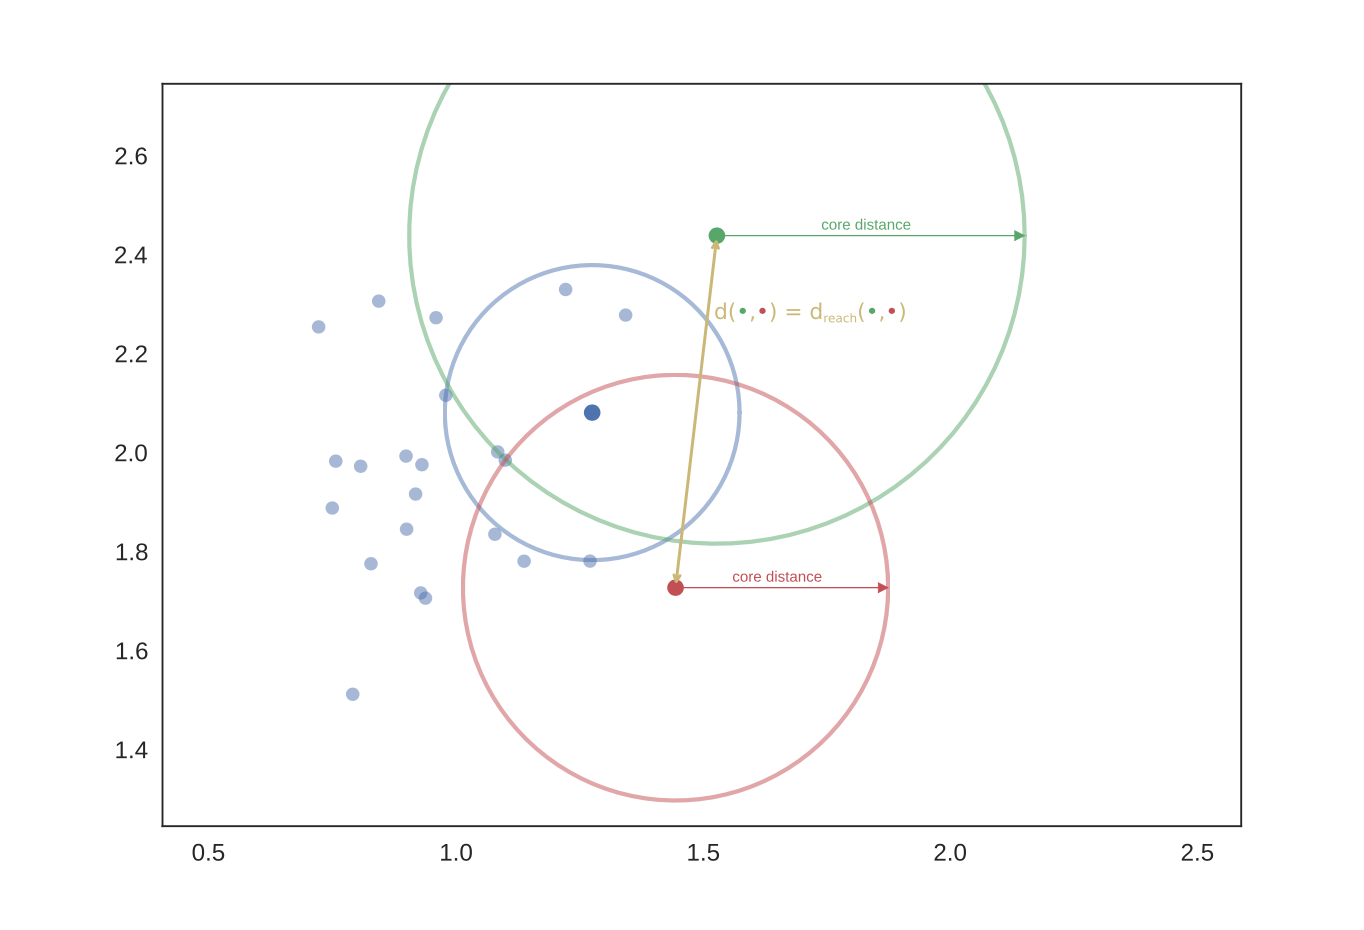
\includegraphics[width=\linewidth]{dis_figure2.png}
		\caption{}
	\end{subfigure}
\end{figure}

\end{frame}

\begin{frame}{Condense tree}
\begin{itemize}
	\item If left child cluster point number is greater than minimum cluster size, but right side is not, Figure(a), keep the left branch and ignore right cluster;
	\item If left and right child clusters are both greater than minimum cluster size, Figure(b), we consider that a cluster split and let the split persist the whole tree;
	\item If left and right child clusters are both fewer than minimum cluster size, Figure(c), we ignore the two cluster.
\end{itemize}
\begin{figure}[h!]
	\centering
	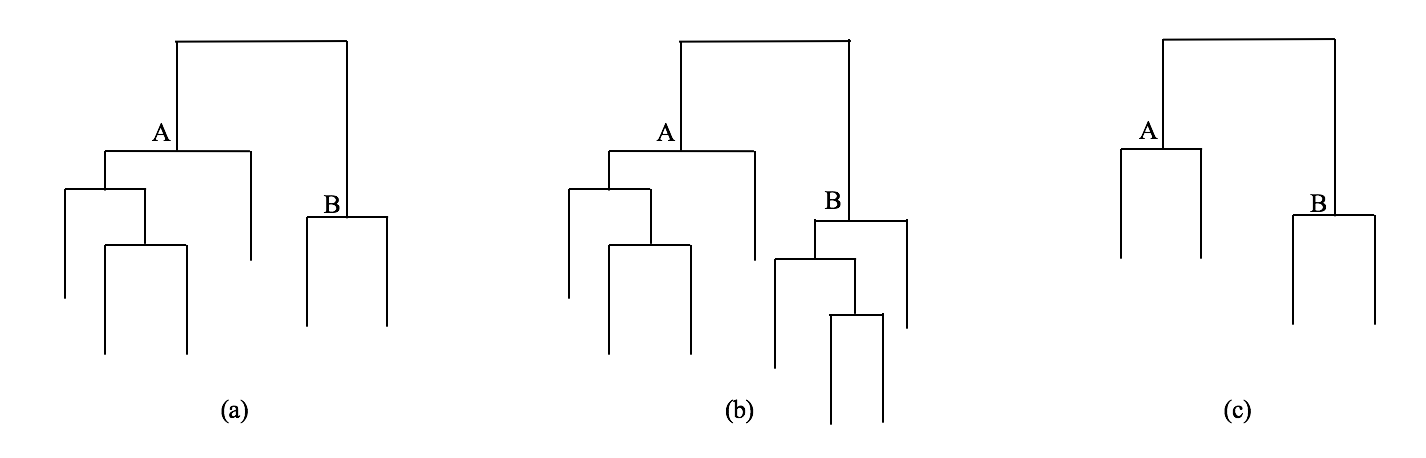
\includegraphics[scale=0.45]{b.png}
\end{figure}
\end{frame}

\begin{frame}{Condense tree algorithm}
\tiny
\begin{algorithm}[H]
	\SetAlgoNoLine
	\SetKwData{minClusterSize}{minClusterSize}
	\SetKwData{numPoints}{numPoints}
	\SetKwData{left}{left}
	\SetKwData{leftCount}{leftCount}
	\SetKwData{right}{right}
	\SetKwData{rightCount}{rightCount}
	\SetKwData{p}{p}
	\SetKwData{tmpNode}{tmpNode}
	\SetKwArray{nodeList}{nodeList}
	\SetKwArray{H}{H}
	\SetKwArray{T}{T}
	\SetKwArray{nextLabel}{nextLabel}
	\SetKwFunction{BFS}{BFS}
	\KwIn{\H{$m$} $\leftarrow$ hierarchy tree}
	\KwOut{\T{$n$} $\leftarrow$ condense tree}
	\nodeList $\leftarrow$ \BFS{$H$}\;
	\For{$r \leftarrow 0$ \KwTo $m$}{
		\If{\nodeList{r} is ignored} {Pass\;}
		\left $\leftarrow$ \nodeList{r}.child1\;
		\leftCount  $\leftarrow$ \H{\left}.childrenSize\;
		\right $\leftarrow$ \nodeList{r}.child2\;
		\rightCount  $\leftarrow$ \H{\right}.childrenSize\;
		\If{\leftCount $\geq$ \minClusterSize \textbf{and} \rightCount $\geq$ \minClusterSize}{
			\T{{\p}$++$} $\leftarrow$ (\nextLabel, $++${\nextLabel}, $1/\mathrm{distance}$, \leftCount);
			\T{{\p}$++$} $\leftarrow$ (\nextLabel, $++${\nextLabel}, $1/\mathrm{distance}$, \rightCount)\;
		}
		\If{\leftCount $<$ \minClusterSize}{
			\For{\tmpNode \textbf{in} \BFS{\left}}{
				\If{\tmpNode is leaf}{
					\T{{\p}$++$} $\leftarrow$ (\nextLabel, \tmpNode, $1/\mathrm{distance}$, $1$)\;
				}
				Ignore \tmpNode\;
			}
		}
		\If{\rightCount $<$ \minClusterSize}{
			\For{\tmpNode \textbf{in} \BFS{\right}}{
				\If{\tmpNode is leaf}{
					\T{{\p}$++$} $\leftarrow$ (\nextLabel, \tmpNode, $1/\mathrm{distance}$, $1$)\;
				}
				Ignore \tmpNode\;
			}
		}
	}
\end{algorithm}
\end{frame}

\begin{frame}{Cluster stability}
\begin{definition}
	Let $\lambda = \frac{1}{d_{\mathrm{mrd}_k}}$. For each cluster we give $\lambda_{\mathrm{birth}}$ and $\lambda_p$ to be the lambda value when the cluster split off then became it’s own cluster, and the lambda value (if any) when the cluster split into smaller clusters respectively.
\end{definition}
$$ S(C) = \sum_{p \in {C}} (\lambda_p - \lambda_{\mathrm{birth}})$$
\end{frame}

\begin{frame}{Cluster stability algorithm}
\begin{algorithm}[H]
	\SetAlgoNoLine
	\SetKwArray{birthLambda}{birth$\lambda$}
	\SetKwData{currChild}{currChild}
	\SetKwData{prevChild}{prevChild}
	\SetKwData{currLambda}{curr$\lambda$}
	\SetKwData{minLambda}{min$\lambda$}
	\SetKwFunction{Min}{Min}
	\SetKwArray{T}{T}
	\SetKwArray{S}{S}
	\KwIn{\T{$n$} $\leftarrow$ condense tree in reverse topological order contains a tuple of (parent,child,$\lambda$,childrenSize)}
	\KwOut{\S{$n$} $\leftarrow$  stability of every node in condense tree}
	\For{$r \leftarrow 0$ \KwTo $n$}{
		\currChild $\leftarrow$ \T{$r$}.child\;
		\currLambda $\leftarrow$ \T{$r$}.$\lambda$\;
		\eIf{\currChild $=$ \prevChild}{
			\minLambda $\leftarrow$ \Min{\minLambda, \currLambda}\;
		}{
			\birthLambda{\currChild} $\leftarrow$ \minLambda\;
			\prevChild $\leftarrow$ \currChild\;
			\minLambda $\leftarrow$ \currLambda\;
		}
	}
	\For{$r \leftarrow 0$ \KwTo $n$}{
		$\S{r} \leftarrow \S{r} + \T{r}.\lambda - $\birthLambda{\T{r}.$\mathrm{parent}$} $\times \T{r}. \mathrm{childrenSize}$ \;
	}
\end{algorithm}
\end{frame}

\begin{frame}{Flat clustering}
\begin{definition}
	Set $SC(C)$ is the sum of the stabilities of the child cluster of cluster $C$.
	$$SC(C) = \sum_{q \in C}S(c)$$
\end{definition}
\end{frame}

\begin{frame}{Flat clustering algorithm}
\begin{algorithm}[H]
	\SetAlgoNoLine
	\SetKwData{subtreeStabilities}{subtreeStabilities}
	\SetKwData{childList}{childList}
	\SetKwData{tmpNode}{tmpNode}
	\SetKwFunction{Bfs}{Bfs}
	\SetKwArray{S}{S}
	\SetKwArray{L}{L}
	\KwIn{\S{$n$} $\leftarrow$  stability condense tree sorted in reverse topological order}
	\KwOut{\L{$n$} $\leftarrow$ \textbf{True} cluster is selected; \textbf{False} otherwise}
	\L $\leftarrow$ \{\textbf{True}\}\;
	\For{$r \leftarrow 0$ \KwTo $n$}{
		\childList $\leftarrow$ \{list of node whose parent is $r$\}\;
		\subtreeStabilities $\leftarrow$ $\sum_{c \in \childList} \S{c}$\;
		\eIf{\subtreeStabilities $>$ \S{$r$}}{
			\L{$r$} $\leftarrow$ \textbf{False}\;
			\S{$r$} $\leftarrow$ \subtreeStabilities\;
		}{
			\For{\tmpNode \textbf{in} \BFS{$r$}}{
				\If{\tmpNode $\neq r$}{\L{\tmpNode} $\leftarrow$ \textbf{False}}
			}
		}
	}
	\caption{Abstract cluster with stabilities}
\end{algorithm}
\end{frame}

\begin{frame}{Experiment}
\begin{figure}[h!]
	\begin{subfigure}{.5\textwidth}
		\centering
		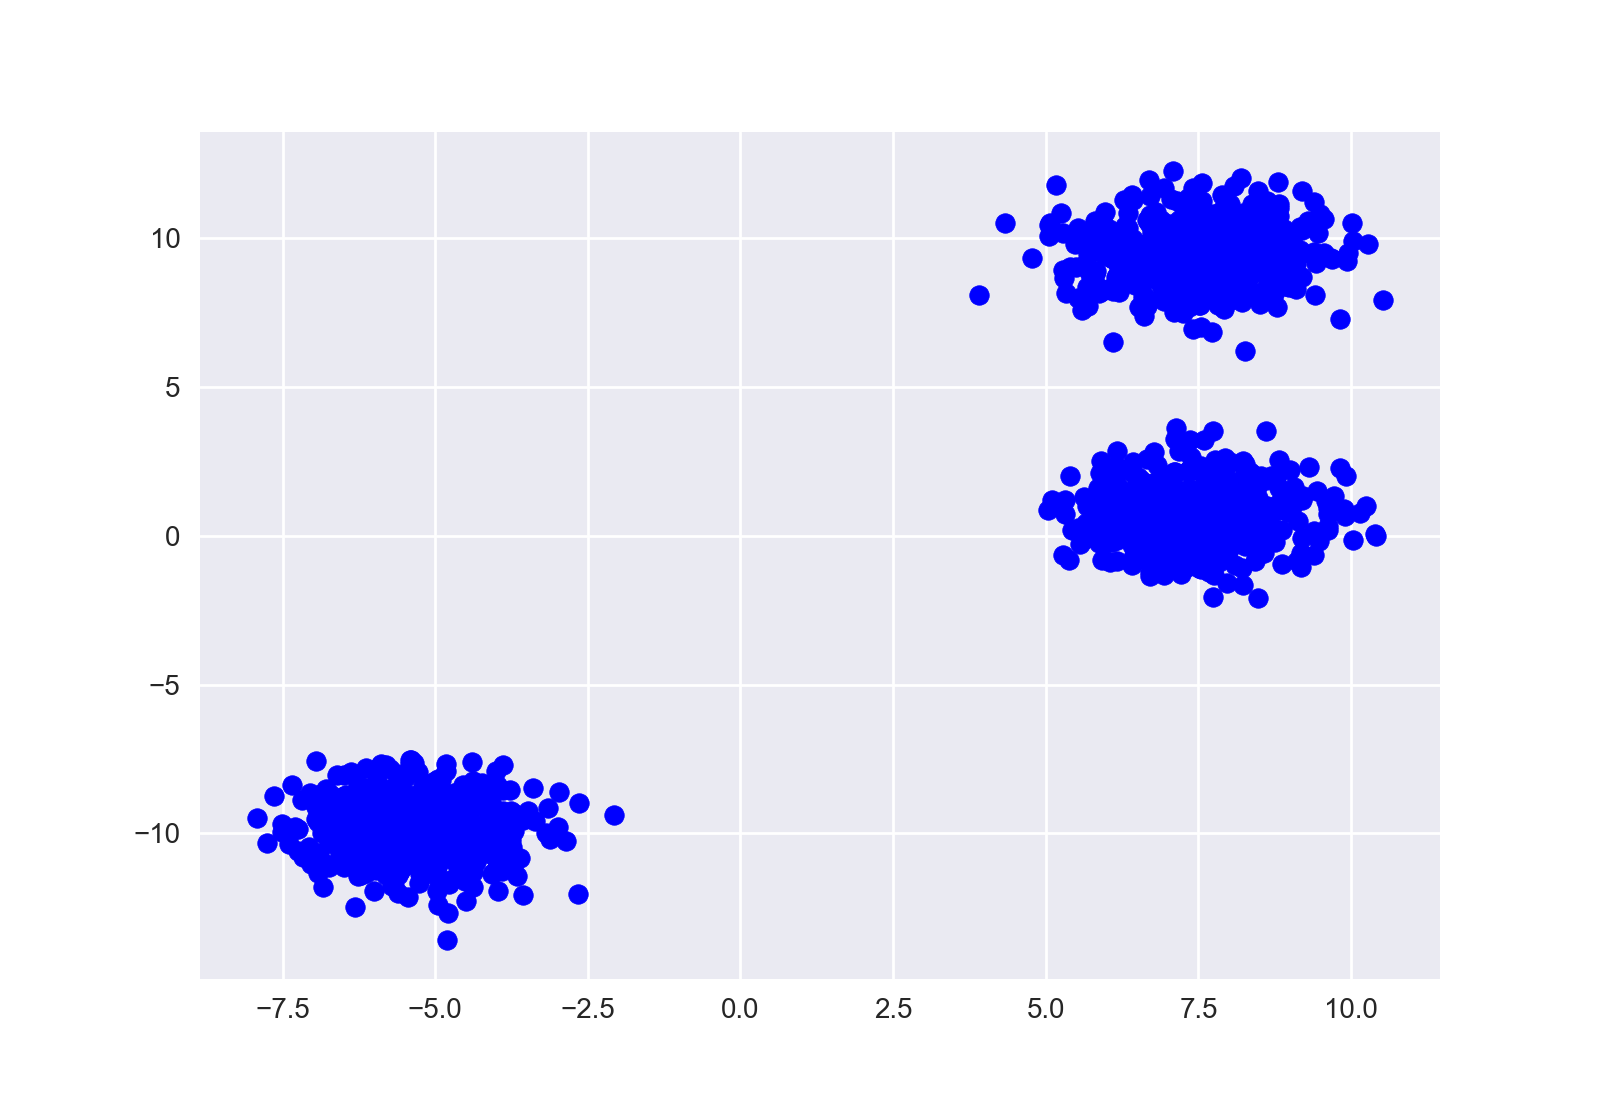
\includegraphics[width=.8\linewidth]{b_figure_1.png}
	\end{subfigure}%
	\begin{subfigure}{.5\textwidth}
		\centering
		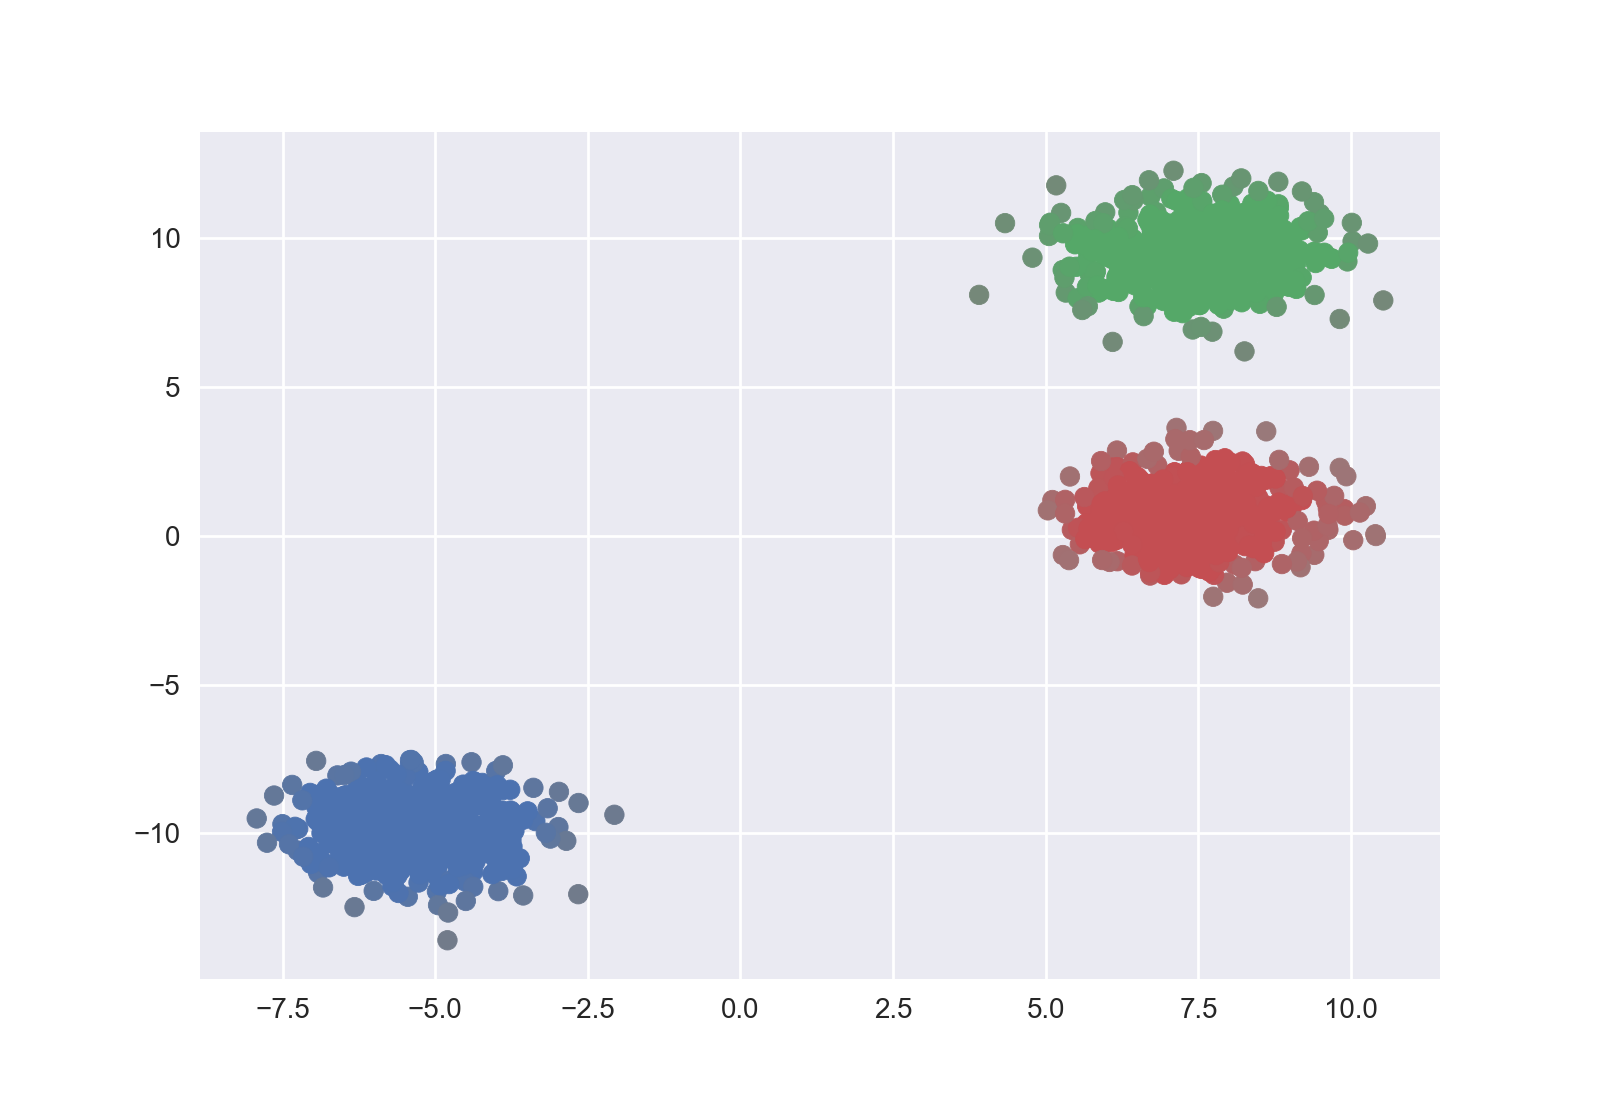
\includegraphics[width=.8\linewidth]{b_figure_2.png}
	\end{subfigure}
\end{figure}
\begin{figure}[h!]
	\begin{subfigure}{.5\textwidth}
		\centering
		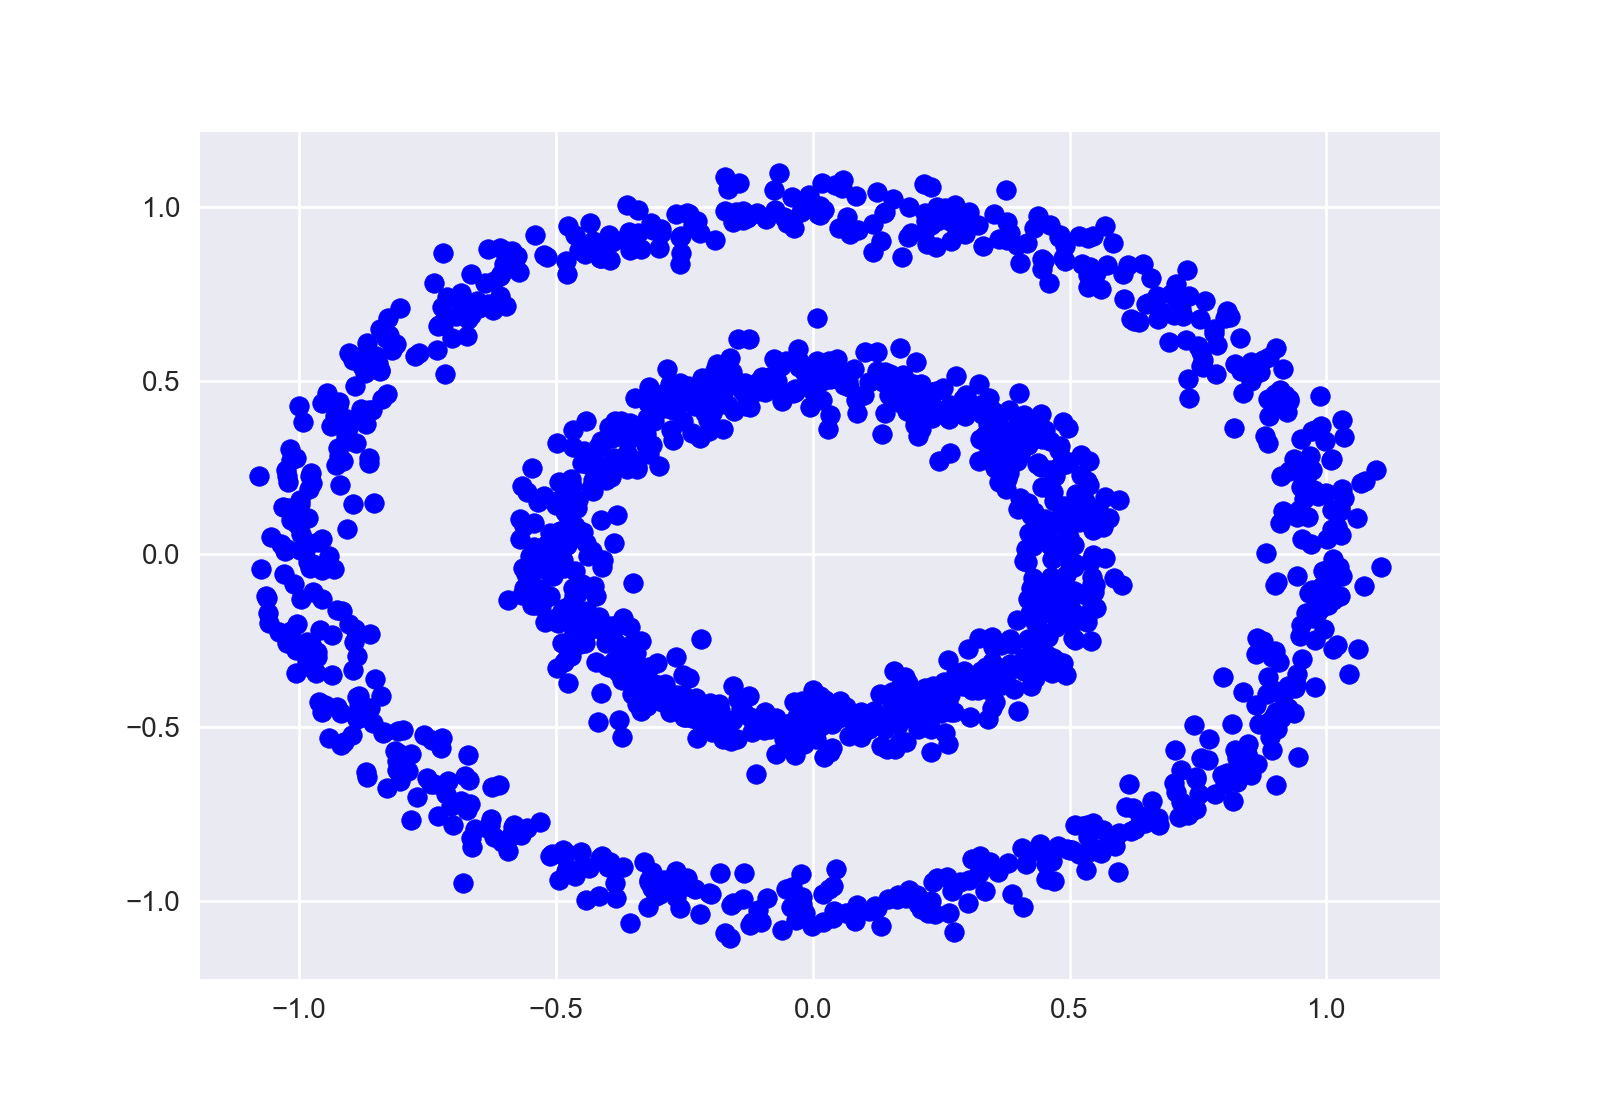
\includegraphics[width=.8\linewidth]{c_figure_1.png}
	\end{subfigure}%
	\begin{subfigure}{.5\textwidth}
		\centering
		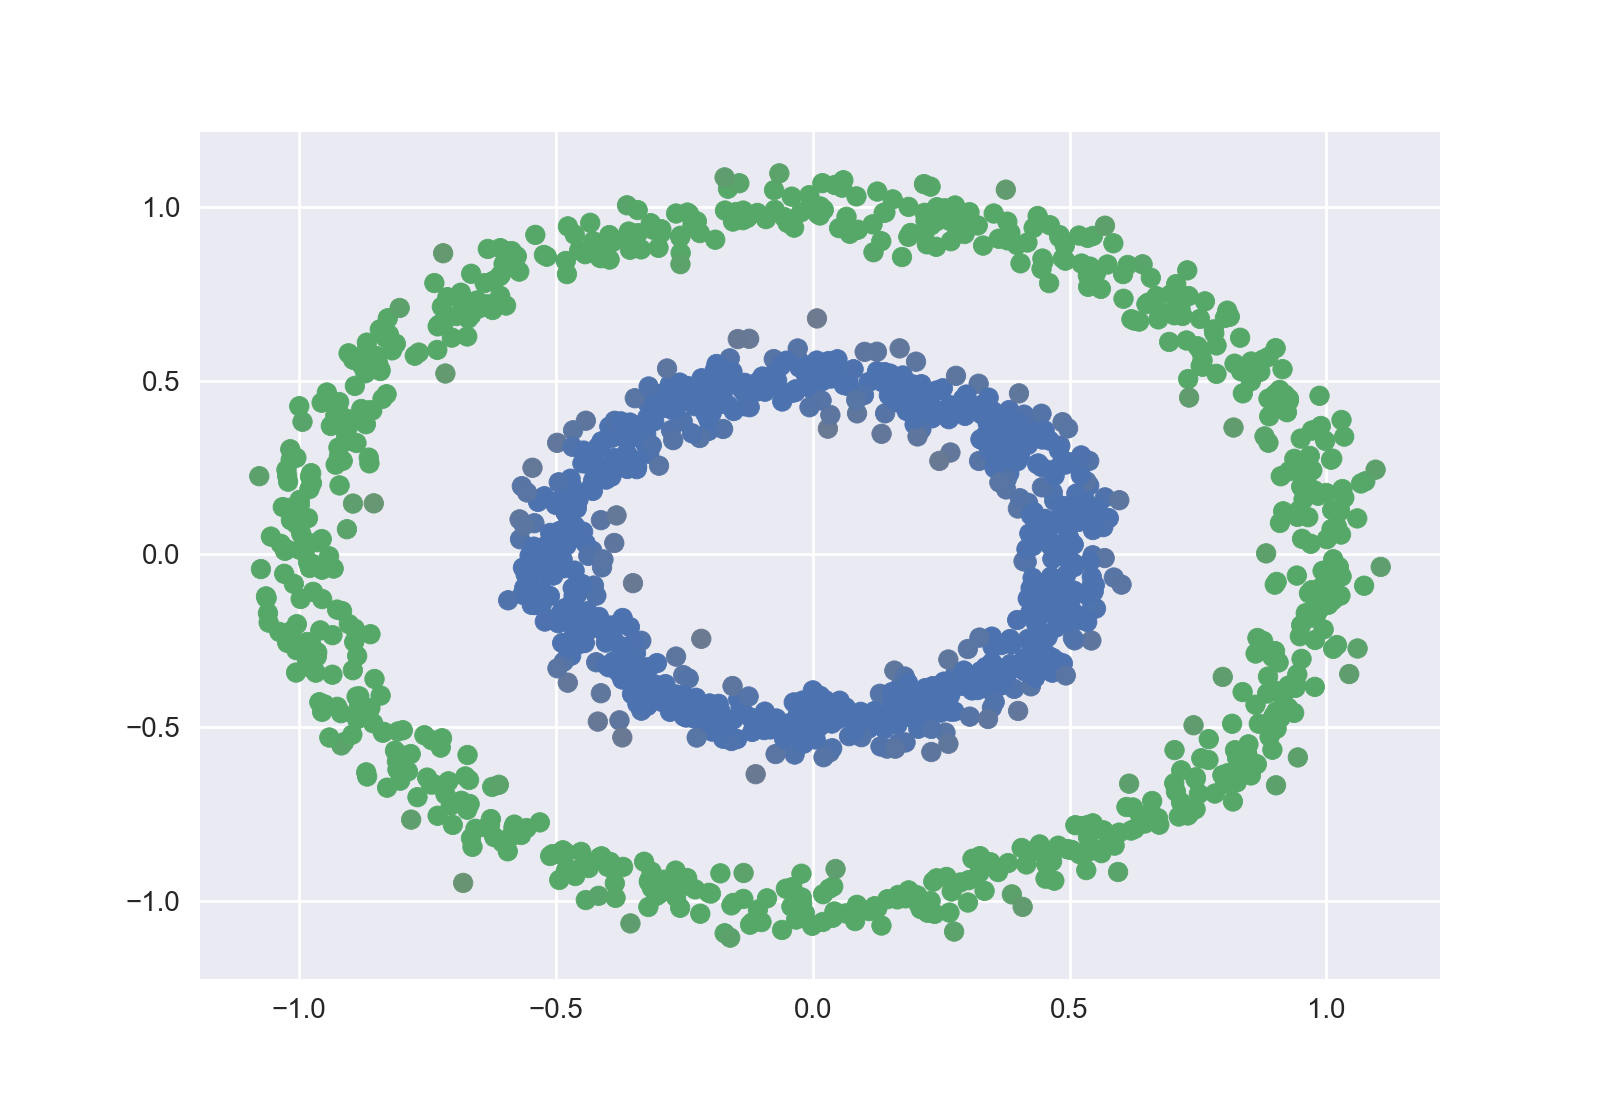
\includegraphics[width=.8\linewidth]{c_figure_2.png}
	\end{subfigure}
\end{figure}
\end{frame}

\begin{frame}{Experiment (cont.)}
\begin{figure}[h!]
	\begin{subfigure}{.5\textwidth}
		\centering
		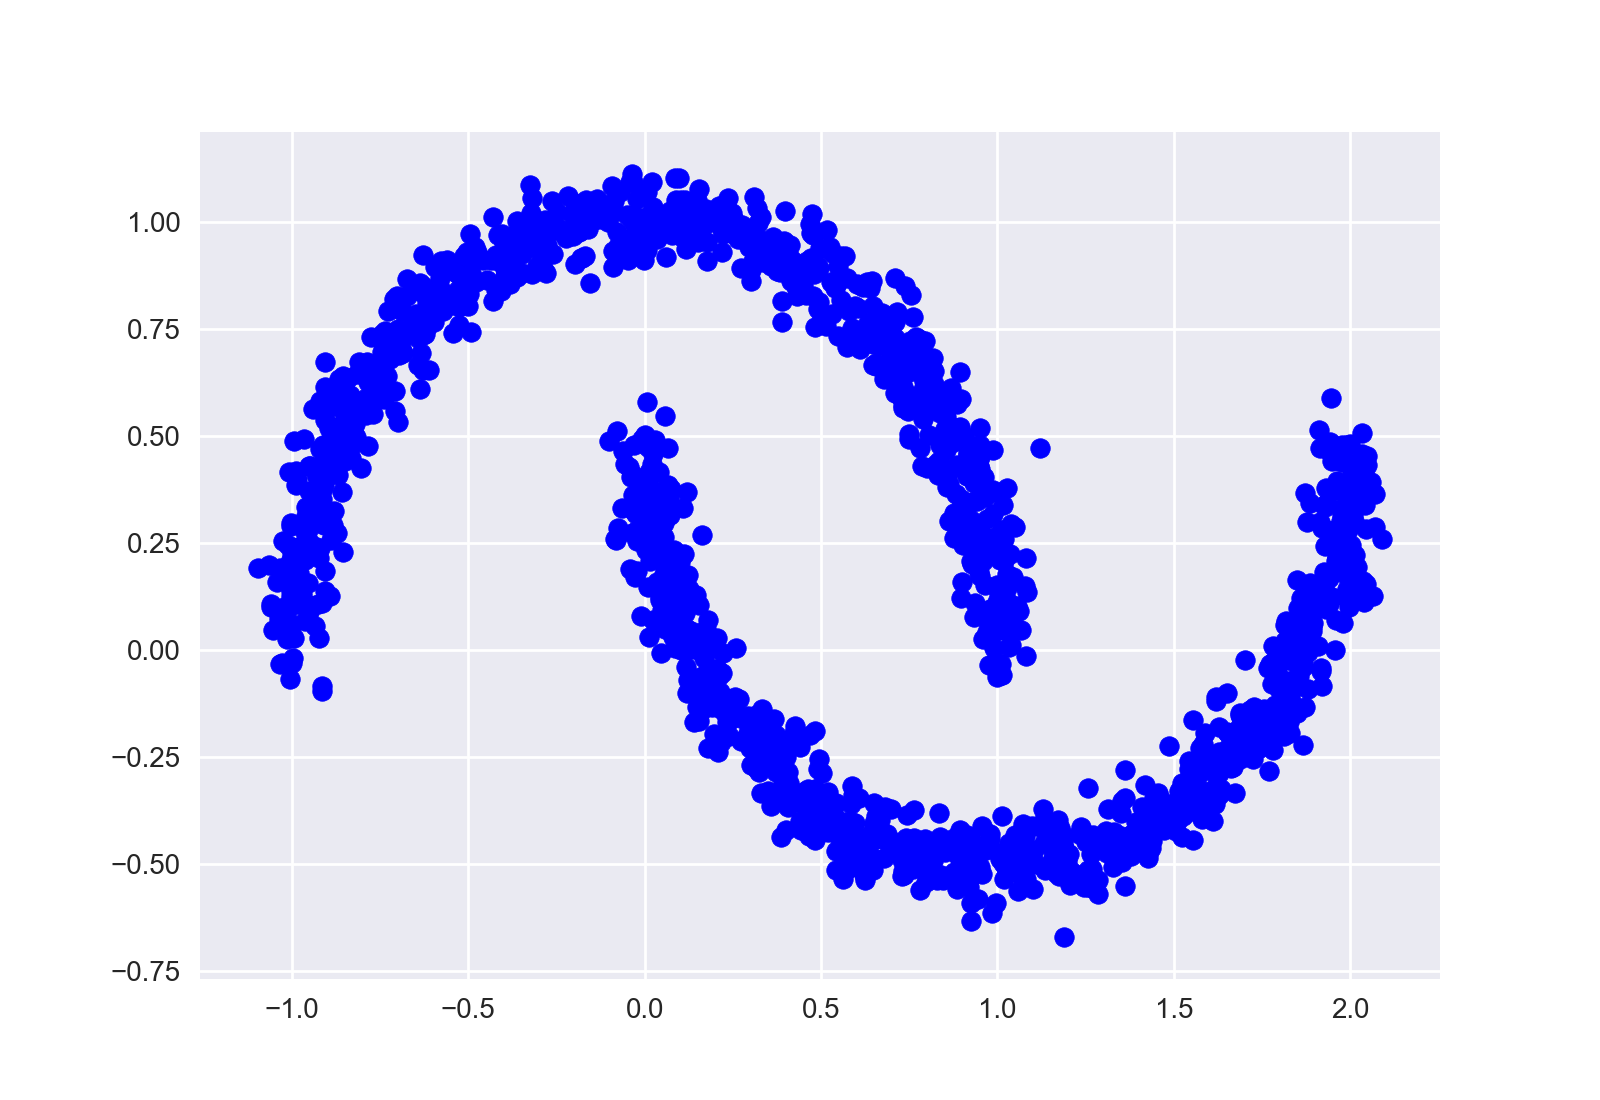
\includegraphics[width=.8\linewidth]{m_figure_1.png}
	\end{subfigure}%
	\begin{subfigure}{.5\textwidth}
		\centering
		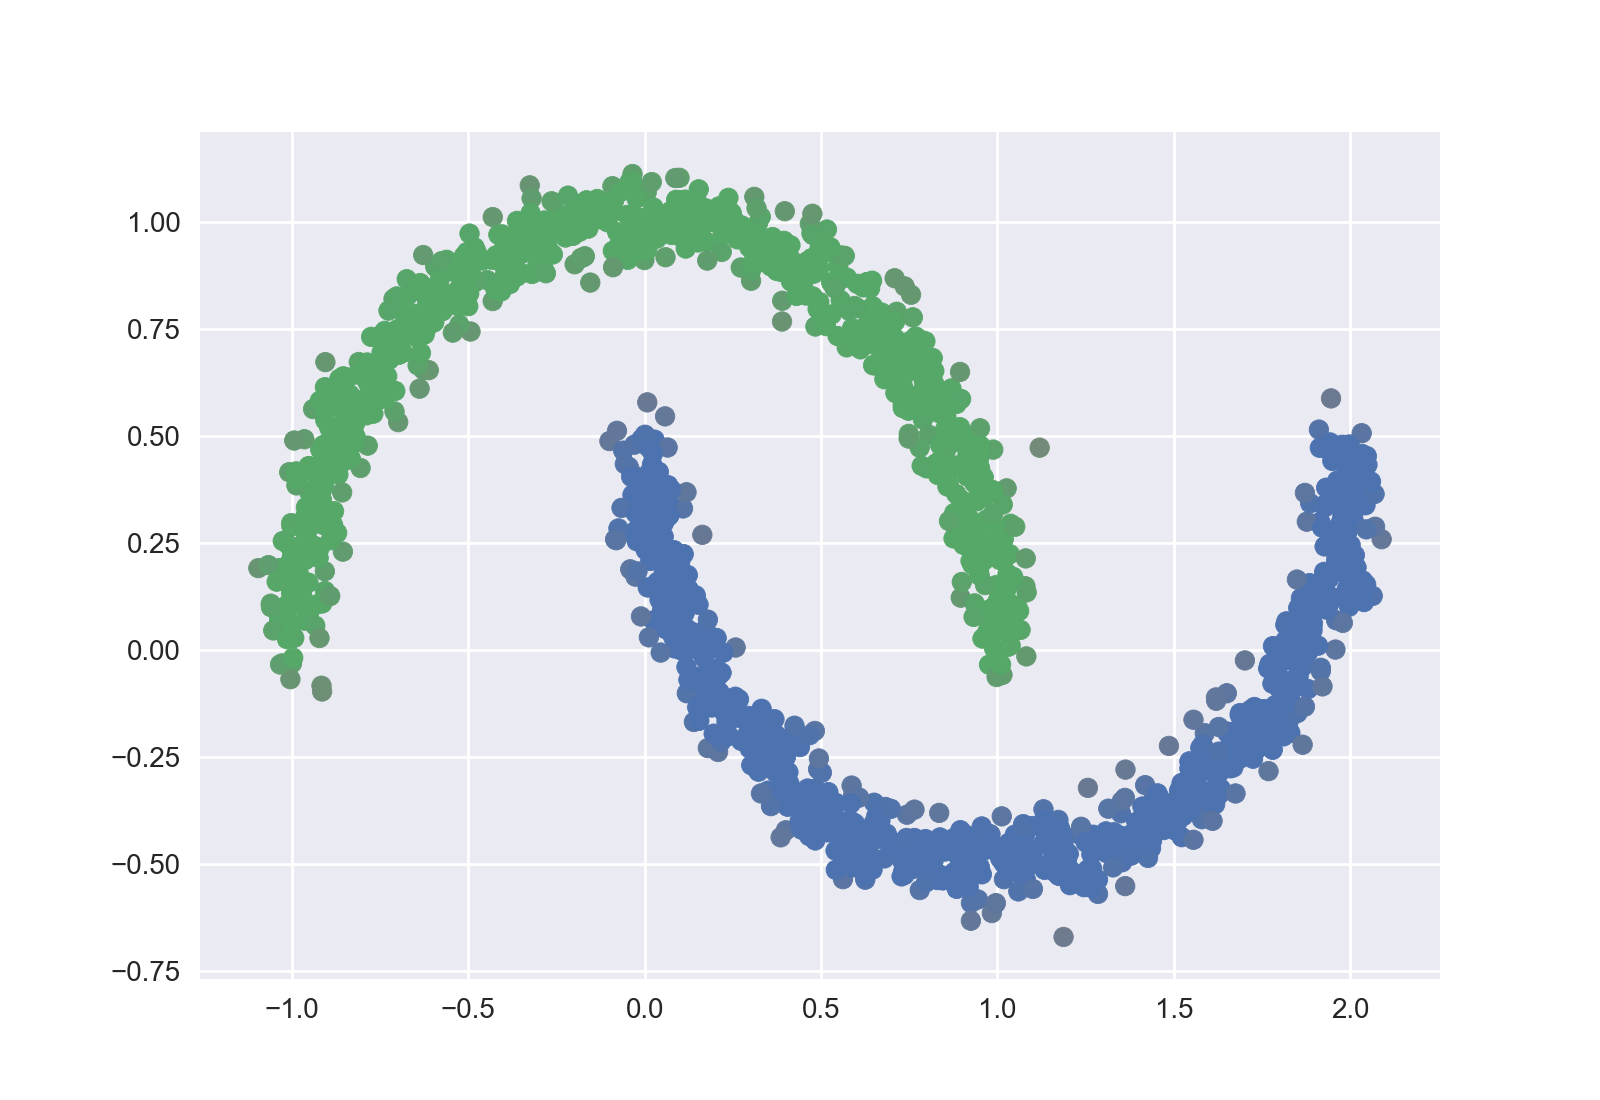
\includegraphics[width=.8\linewidth]{m_figure_2.png}
	\end{subfigure}
\end{figure}
\begin{figure}[h!]
	\begin{subfigure}{.5\textwidth}
		\centering
		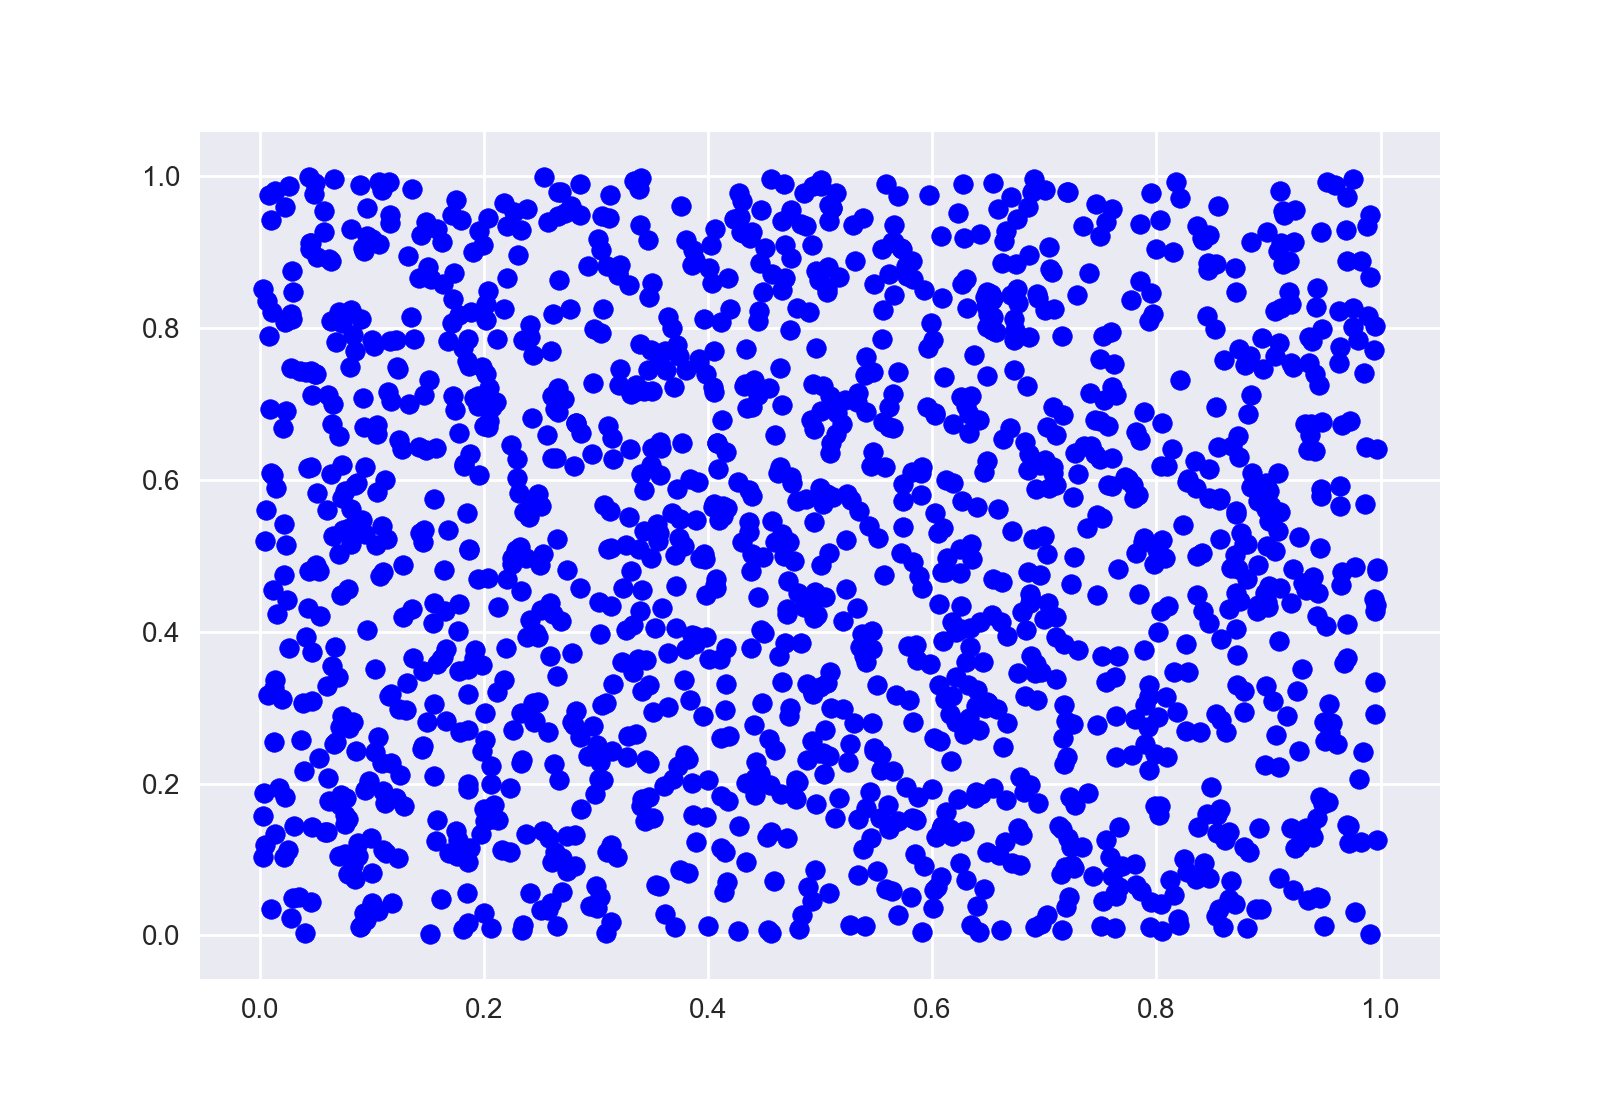
\includegraphics[width=.8\linewidth]{r_figure_1.png}
	\end{subfigure}%
	\begin{subfigure}{.5\textwidth}
		\centering
		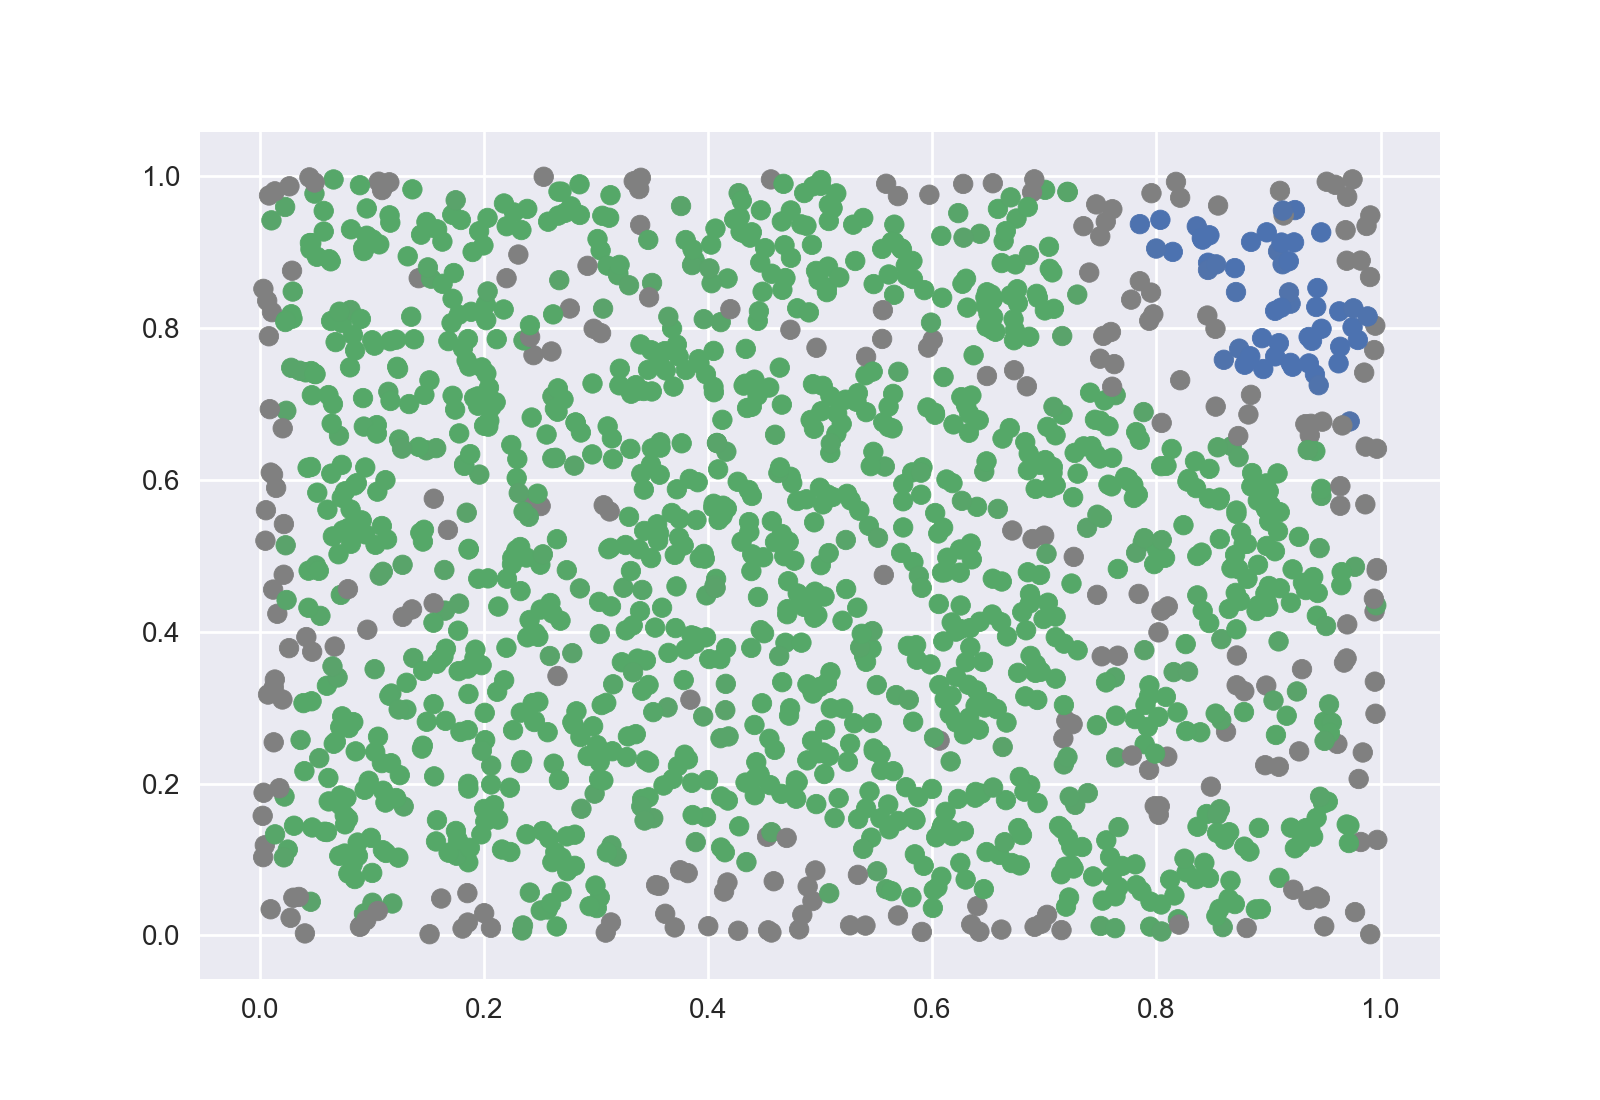
\includegraphics[width=.8\linewidth]{r_figure_2.png}
	\end{subfigure}
\end{figure}
\end{frame}

\begin{frame}{Experiment (cont.)}

\begin{figure}[h!]
	\centering
	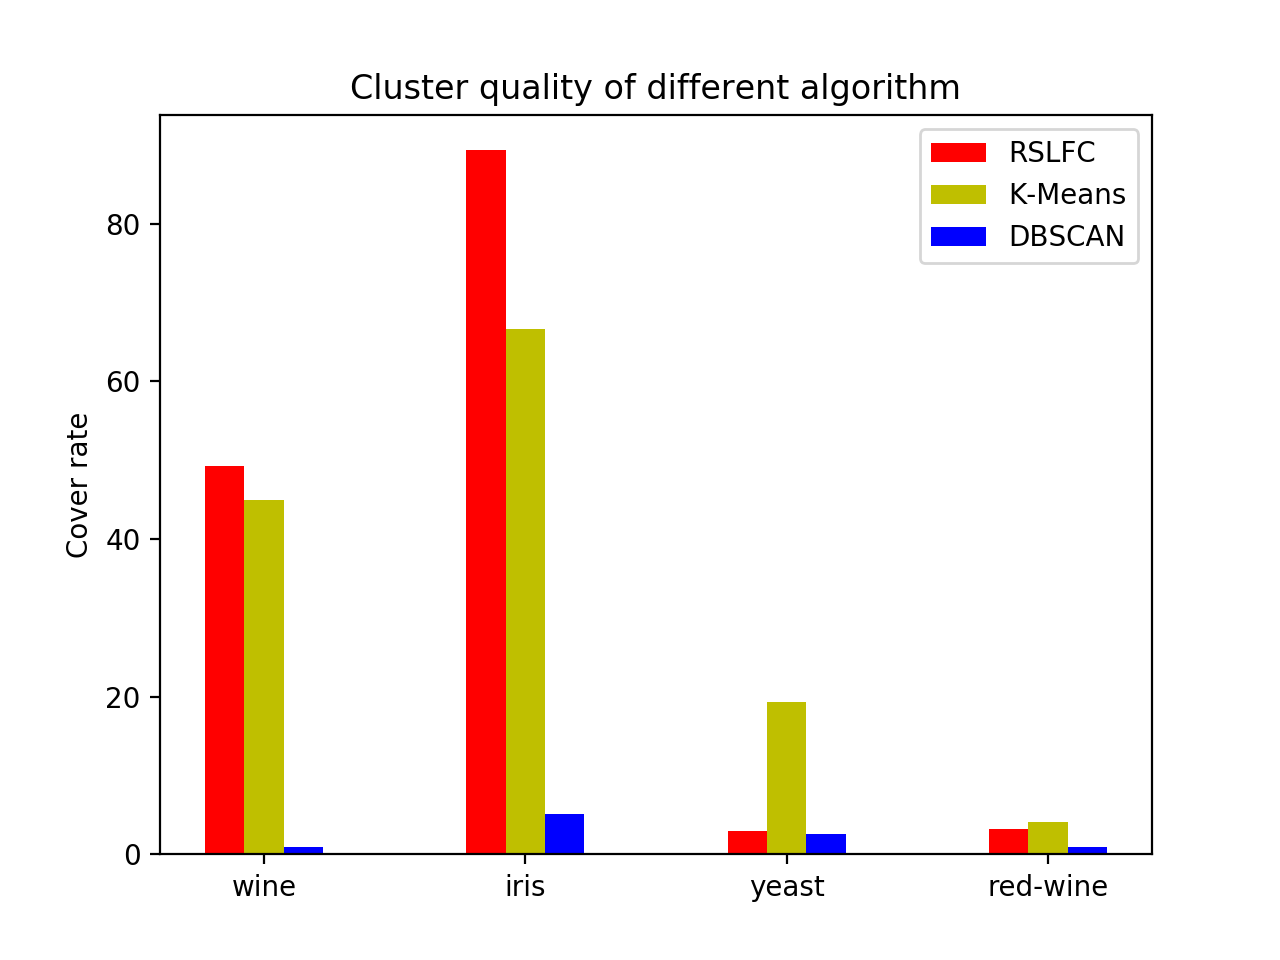
\includegraphics[scale=0.6]{hist1.png}
\end{figure}

\end{frame}

\begin{frame}{References}


\frametitle{References}
\nocite{chaudhuri2010rates, campello2013density, McInnes2017}
\bibliographystyle{apacite}
\bibliography{mybib.bib}
\end{frame}
\end{document}